\documentclass[11pt]{article}

\usepackage[a4paper,margin=20mm,headheight=15pt]{geometry}
\usepackage{fontspec}
\usepackage{unicode-math}
\setmainfont{texgyrepagella-regular.otf}[
  Path=/usr/local/texlive/2024/texmf-dist/fonts/opentype/public/tex-gyre/,
  BoldFont=texgyrepagella-bold.otf,
  ItalicFont=texgyrepagella-italic.otf,
  BoldItalicFont=texgyrepagella-bolditalic.otf
]
\setmathfont{texgyrepagella-math.otf}[
  Path=/usr/local/texlive/2024/texmf-dist/fonts/opentype/public/tex-gyre-math/
]

\usepackage[final]{microtype}
\usepackage{xcolor}
\usepackage{booktabs}
\usepackage{tabularx}
\usepackage{array}
\usepackage{enumitem}
\usepackage{titlesec}
\usepackage{fancyhdr}
\usepackage[most]{tcolorbox}
\usepackage{tikz}
\usetikzlibrary{arrows.meta,positioning}
\usepackage{hyperref}

\definecolor{navy}{HTML}{17324D}
\definecolor{blue}{HTML}{346B91}
\definecolor{teal}{HTML}{357E78}
\definecolor{gold}{HTML}{B5842E}
\definecolor{plum}{HTML}{76566F}
\definecolor{ink}{HTML}{25313A}
\definecolor{paper}{HTML}{F7F4ED}
\definecolor{paleBlue}{HTML}{EAF1F6}
\definecolor{paleTeal}{HTML}{E8F2F0}
\definecolor{paleGold}{HTML}{F8F0DE}
\definecolor{palePlum}{HTML}{F2ECF1}
\definecolor{line}{HTML}{CBD5DD}

\hypersetup{
  colorlinks=true,
  linkcolor=navy,
  urlcolor=blue,
  pdftitle={Basic Concepts of String Theory: A 28-Week Seminar Plan},
  pdfauthor={Codex}
}

\setlength{\parindent}{0pt}
\setlength{\parskip}{5pt}
\setlist[itemize]{leftmargin=1.5em,itemsep=2pt,topsep=3pt}
\setlist[enumerate]{leftmargin=1.8em,itemsep=2pt,topsep=3pt}
\renewcommand{\arraystretch}{1.17}

\titleformat{\section}
  {\Large\bfseries\color{navy}}
  {\thesection}{0.6em}{}
  [\vspace{-2pt}\color{line}\titlerule]
\titleformat{\subsection}
  {\large\bfseries\color{blue}}
  {\thesubsection}{0.55em}{}
\titleformat{\subsubsection}
  {\normalsize\bfseries\color{teal}}
  {}{0pt}{}

\pagestyle{fancy}
\fancyhf{}
\lhead{\color{navy}\small \emph{Basic Concepts of String Theory} seminar}
\rhead{\color{navy}\small 28-week plan}
\cfoot{\color{navy}\thepage}
\renewcommand{\headrulewidth}{0.4pt}

\newtcolorbox{keybox}[1][]{
  enhanced,breakable,
  colback=paleBlue,colframe=blue,
  boxrule=0.6pt,arc=2mm,
  left=3mm,right=3mm,top=2mm,bottom=2mm,
  title=#1,fonttitle=\bfseries
}

\newtcolorbox{checkpoint}[1][]{
  enhanced,breakable,
  colback=paleTeal,colframe=teal,
  boxrule=0.6pt,arc=2mm,
  left=3mm,right=3mm,top=2mm,bottom=2mm,
  title=#1,fonttitle=\bfseries
}

\newtcolorbox{warningbox}[1][]{
  enhanced,breakable,
  colback=paleGold,colframe=gold,
  boxrule=0.6pt,arc=2mm,
  left=3mm,right=3mm,top=2mm,bottom=2mm,
  title=#1,fonttitle=\bfseries
}

\newcommand{\core}{\textcolor{navy}{\textbf{Core}}}
\newcommand{\survey}{\textcolor{plum}{\textbf{Survey}}}
\newcommand{\essential}[1]{\textcolor{teal}{\textbf{#1}}}
\newcommand{\roadarrow}{\textcolor{gold}{\ensuremath{\;\longrightarrow\;}}}

\newcommand{\seminarweek}[7]{%
  \begin{tcolorbox}[
    enhanced,
    colback=white,colframe=navy,
    boxrule=0.65pt,arc=1.5mm,
    left=3mm,right=3mm,top=2mm,bottom=2mm,
    title={#1\hfill\normalfont #2},
    fonttitle=\bfseries,coltitle=white,colbacktitle=navy
  ]
  \textbf{Reading.} #3

  \textbf{Main idea.} #4

  \textbf{Seminar road map.} #5

  \textbf{Preparation and output.} #6

  \textbf{Useful references.} #7
  \end{tcolorbox}
}

\begin{document}
\pagenumbering{roman}
\hypersetup{pageanchor=false}

\begin{titlepage}
\pagecolor{paper}
\color{ink}
\vspace*{15mm}

{\color{gold}\rule{\textwidth}{1.2pt}}
\vspace{8mm}

{\Huge\bfseries\color{navy}
\emph{Basic Concepts of String Theory}}

\vspace{3mm}
{\LARGE\color{blue}A 28-week seminar plan}

\vspace{9mm}
{\Large Two semesters $\times$ 14 weeks $\times$ 2 hours}

\vspace{13mm}

\begin{keybox}[Design principle]
The seminar should not attempt to reproduce every line of a 775-page graduate
textbook on the board.  Its job is to expose the logical spine, work the
derivations that newcomers cannot reliably reconstruct alone, and teach
participants how to recover the remaining details from the book.
\end{keybox}

\vfill

\begin{tabularx}{\textwidth}{@{}>{\bfseries\color{navy}}p{34mm}X@{}}
Primary text & R. Blumenhagen, D. L\"ust, and S. Theisen,
\emph{Basic Concepts of String Theory} (Springer, 2013) \tabularnewline
Audience & Beginning graduate students with quantum mechanics, introductory
QFT, special relativity, and some general relativity; prior string theory is not
assumed \tabularnewline
Meeting time & Two hours per week \tabularnewline
Expected preparation & Varies strongly by background and purpose; see the four
participant profiles in Sec.~1.2 \tabularnewline
Coverage strategy & Derive the structural results in full; discuss long model
lists, appendices, and specialized examples at survey level \tabularnewline
End point & A coherent path from the Polyakov string and worldsheet CFT to
compactification, D-branes, fluxes, dualities, M-theory, F-theory, and AdS/CFT
\end{tabularx}

\vspace{8mm}
{\color{gold}\rule{\textwidth}{1.2pt}}
\end{titlepage}
\nopagecolor
\hypersetup{pageanchor=true}

\tableofcontents
\clearpage
\pagenumbering{arabic}

\section{Pacing assumptions}

\begin{warningbox}[Page-number convention]
All page numbers in this plan are the \emph{printed} page numbers in the book,
not the PDF viewer's page count.  The offset is not constant throughout the PDF,
so use chapter and section titles as the definitive locator.
\end{warningbox}

For a newcomer, this book is normally read at about five to eight serious pages
per hour once equations are reconstructed.  Thus a 25-page assignment is not a
two-hour task: it is a four-to-six-hour preparation task.  The seminar itself is
where the group checks the conceptual map and two or three difficult steps.

\subsection{Core versus survey coverage}

Each week has two implicit levels:

\begin{itemize}
  \item \core{} material should be understood well enough to reproduce the
  assumptions, derivation, and physical meaning.  It receives board time.
  \item \survey{} material should be read for structure, examples, and notation.
  The speaker states the result and its role but does not derive every formula.
\end{itemize}

This distinction is what makes full-book coverage possible in 28 meetings.
Without it, a careful seminar would need at least three semesters.

In every weekly road map below, the \essential{teal bold node} is the result or
derivation that should survive even if discussion runs slowly.  The arrows show
logical dependence, not a rigid timetable.

\subsection{Expected time cost for different participants}

The common cost is the two-hour meeting.  The estimates below are additional
weekly preparation time; advanced compactification weeks can require the upper
end of each range.

\begin{itemize}[leftmargin=0pt,label={},itemsep=8pt]
  \item \textbf{Fresh participant intending to do research in string theory: 7--11 hours outside the seminar.}
  Read all \core{} material and most \survey{} material, reconstruct the main
  derivation, and solve the weekly exercise.  During BRST, superconformal CFT,
  Calabi--Yau compactification, and duality weeks, 10--13 hours is realistic.
  This participant should take speaker and checker roles regularly.

  \item \textbf{Fresh participant exploring the field: 3--5 hours outside the seminar.}
  Read the chapter introduction, the \core{} subsections, and the closing
  discussion; follow one derivation carefully and treat the rest as orientation.
  Exercises are optional but strongly recommended in Weeks 2--9 and 11--15,
  where later material depends directly on the foundations.

  \item \textbf{Very fresh participant, including someone with limited QFT background: 2--4 hours for attendance, or 7--12 hours for technical progress.}
  The lighter track consists of a conceptual preview and vocabulary sheet; it
  is enough to attend profitably but not to master the derivations.  The
  technical track adds 3--6 hours of foundation repair in QFT, special
  relativity, path integrals, group theory, or differential geometry.  Such a
  participant should not be expected to present BRST, modular invariance, or
  supergravity before completing the relevant bridge material.

  \item \textbf{Participant who has studied string theory once: 3--6 hours outside the seminar.}
  Skim familiar sections, reconstruct the essential derivation from memory,
  and use a second reference to check conventions.  If serving as speaker, add
  roughly 3--5 hours for preparing a coherent road map and anticipating
  questions from newcomers.
\end{itemize}

\begin{keybox}[Role-dependent additions]
Relative to the profile above, allow approximately 3--5 extra hours for the
speaker, 1--2 hours for the checker, and 1--2 hours after the meeting for the
scribe.  These duties should rotate; otherwise the apparent workload of the
seminar will be distributed very unevenly.
\end{keybox}

\begin{checkpoint}[How to calibrate the pace with fresh students]
At the end of Weeks 2, 5, and 8, anonymously ask: (i) preparation hours,
(ii) fraction of the reading understood before the meeting, and (iii) which
derivation remained opaque afterward.  If the median preparation exceeds six
hours, reduce the next assignment's \survey{} portion.  Do not accelerate merely
because the presenter is experienced.
\end{checkpoint}

\subsection{Roles for a participatory seminar}

Use three rotating roles each week:

\begin{itemize}
  \item the \textbf{speaker} prepares the logical map and the main derivation;
  \item the \textbf{checker} independently verifies conventions, signs, and one
  limiting case against a secondary source;
  \item the \textbf{scribe} produces a two-page note containing the final
  equations, unresolved questions, and corrections after discussion.
\end{itemize}

The speaker should circulate a one-page roadmap 24 hours before the meeting.
Slides may be used for geometry, spectra, and summary tables, but the principal
derivation should be done on a board or tablet slowly enough to invite questions.

\section{The two-semester logic}

\begin{center}
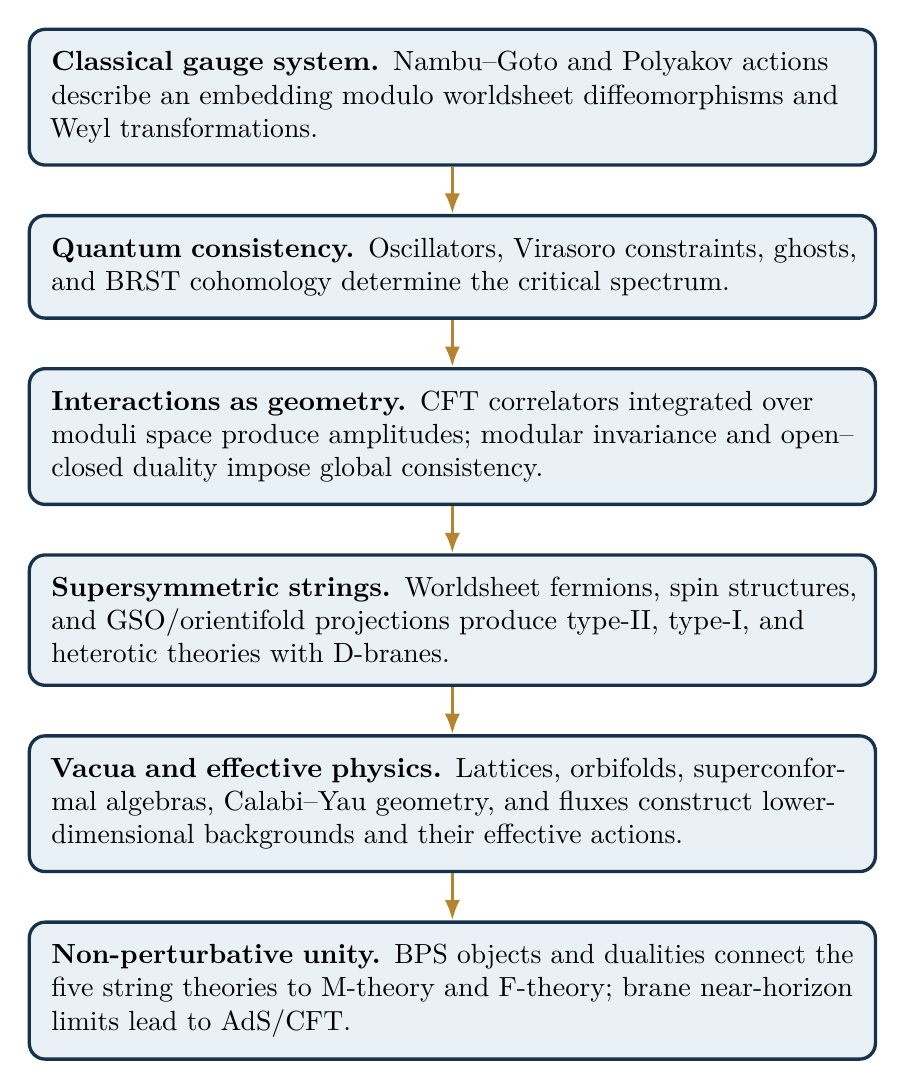
\begin{tikzpicture}[
  node distance=6mm,
  box/.style={rounded corners=2mm,draw=navy,very thick,fill=paleBlue,
    text width=.84\textwidth,minimum height=11mm,align=left,inner sep=2.8mm},
  arr/.style={-{Latex[length=2.6mm]},very thick,draw=gold}
]
\node[box] (a) {\textbf{Classical gauge system.}  Nambu--Goto and Polyakov
actions describe an embedding modulo worldsheet diffeomorphisms and Weyl
transformations.};
\node[box,below=of a] (b) {\textbf{Quantum consistency.}  Oscillators,
Virasoro constraints, ghosts, and BRST cohomology determine the critical
spectrum.};
\node[box,below=of b] (c) {\textbf{Interactions as geometry.}  CFT correlators
integrated over moduli space produce amplitudes; modular invariance and
open--closed duality impose global consistency.};
\node[box,below=of c] (d) {\textbf{Supersymmetric strings.}  Worldsheet
fermions, spin structures, and GSO/orientifold projections produce type-II,
type-I, and heterotic theories with D-branes.};
\node[box,below=of d] (e) {\textbf{Vacua and effective physics.}  Lattices,
orbifolds, superconformal algebras, Calabi--Yau geometry, and fluxes construct
lower-dimensional backgrounds and their effective actions.};
\node[box,below=of e] (f) {\textbf{Non-perturbative unity.}  BPS objects and
dualities connect the five string theories to M-theory and F-theory; brane
near-horizon limits lead to AdS/CFT.};
\draw[arr] (a)--(b); \draw[arr] (b)--(c); \draw[arr] (c)--(d);
\draw[arr] (d)--(e); \draw[arr] (e)--(f);
\end{tikzpicture}
\end{center}

Semester I establishes the first four boxes and ends with the consistent
ten-dimensional superstrings.  Semester II develops the last two boxes.  The
late chapters are not independent decorations: they repeatedly use BRST,
modular invariance, boundary states, and supersymmetry from Semester I.

\clearpage
\section{Semester I: Worldsheet foundations and ten-dimensional strings}

\begin{keybox}[Semester I objective]
By Week 14, participants should be able to explain why the critical dimensions
and spectra arise, how amplitudes are organized by worldsheet topology and
moduli, and how spin structures and projections produce type-II and type-I
superstrings with D-branes.
\end{keybox}

\seminarweek{Week 1}{Chs.~1; 2.1--2.3, pp.~1--22}
{Introduction; relativistic particle; Nambu--Goto and Polyakov actions and their
symmetries.  The particle review is \survey{} if the audience already knows
reparametrization invariance.}
{A relativistic string is a two-dimensional gauge system.  The auxiliary
worldsheet metric makes diffeomorphism and Weyl symmetry manifest, and its
equation of motion imposes $T_{ab}=0$.}
{Motivation and course map \roadarrow Nambu--Goto versus Polyakov
\roadarrow \essential{worldsheet stress tensor, gauge symmetries, and
$T_{ab}=0$} \roadarrow on-shell equivalence of the two actions.}
{Beforehand, vary both actions and list all local/global symmetries.  The scribe
produces a convention sheet for signatures, $\alpha'$, tension, and worldsheet
coordinates.}
{Tong, \emph{Lectures on String Theory}, Sec.~1; Polchinski I, Secs.~1.2--1.3;
Becker--Becker--Schwarz (BBS), Ch.~2.}

\seminarweek{Week 2}{Ch.~2.4--2.5, pp.~23--34}
{Oscillator expansions and representative classical solutions.}
{Boundary conditions select the mode expansion.  The constraints remove
longitudinal excitations and split closed-string motion into left- and
right-movers tied by level matching.}
{Boundary conditions \roadarrow open/closed mode expansions \roadarrow
\essential{Virasoro constraints and level matching} \roadarrow center-of-mass
motion, winding intuition, and representative classical solutions.}
{Reconstruct one expansion without the book and check its canonical dimensions.
The checker verifies signs for Neumann versus Dirichlet boundary terms.}
{Tong, Sec.~1; Zwiebach, \emph{A First Course in String Theory}, classical-string
chapters; Polchinski I, Secs.~1.3--1.4.}

\seminarweek{Week 3}{Ch.~3.1--3.2, pp.~35--45}
{Canonical and light-cone quantization of the bosonic string.}
{Quantization converts modes into oscillators, while light-cone gauge solves
the constraints explicitly and exposes the physical transverse Hilbert space.}
{Canonical brackets \roadarrow oscillator algebra \roadarrow light-cone gauge
\roadarrow \essential{physical transverse Hilbert space} \roadarrow
normal-ordering and Lorentz-anomaly preview.}
{Compute the zero-point energy with a stated regulator.  The speaker must
distinguish a gauge choice, a constraint, and a physical-state condition.}
{Tong, Sec.~2; Polchinski I, Ch.~2 and Sec.~4.1; BBS, Ch.~2.}

\seminarweek{Week 4}{Ch.~3.3--3.5, pp.~46--62}
{Bosonic spectrum, covariant path-integral quantization, and Virasoro algebra.}
{Critical dimension and intercept are quantum consistency conditions.  The
closed-string massless state already contains $G_{\mu\nu}$, $B_{\mu\nu}$, and
$\Phi$, so gravity is unavoidable.}
{First open/closed mass levels \roadarrow \essential{critical dimension,
intercept, and the closed massless fields} \roadarrow Virasoro central extension
\roadarrow Lorentz/no-ghost consistency.}
{Prepare a spectrum table for open and closed strings.  The checker verifies
state counts in $D=26$ and identifies the tachyon's role and limitation.}
{Tong, Sec.~2; Polchinski I, Ch.~4; BBS, Ch.~2.}

\seminarweek{Week 5}{Ch.~4.1, pp.~63--84}
{Core two-dimensional CFT: conformal maps, OPEs, radial quantization,
state--operator correspondence, Ward identities, and Virasoro symmetry.}
{CFT turns local worldsheet dynamics into algebraic data.  OPE coefficients and
conformal weights control both states and amplitudes.}
{Local conformal transformations \roadarrow stress tensor and Ward identities
\roadarrow \essential{$TT$ OPE, Virasoro algebra, and state--operator map}
\roadarrow free-boson example.}
{Every participant computes $T(z)X(w)$ and $T(z)e^{ikX(w)}$.  The scribe begins
a running table of fields, weights $(h,\bar h)$, and central charges.}
{Ginsparg, \emph{Applied Conformal Field Theory}; Di Francesco--Mathieu--S\'en\'echal,
Chs.~4--6; Tong, Sec.~4.}

\seminarweek{Week 6}{Ch.~4.2--4.5, pp.~85--106}
{Closed-string application, boundary CFT, free-boson boundary states, and
crosscap states.}
{Closed strings use two chiral algebras; boundaries glue them and turn a
spacetime brane into a worldsheet state.  Crosscaps encode orientation reversal.}
{Closed-string vertex conditions \roadarrow conformal gluing \roadarrow
\essential{Neumann/Dirichlet boundary states and their spacetime meaning}
\roadarrow Ishibashi/Cardy preview \roadarrow crosscap conditions.}
{Derive the oscillator gluing condition for one boundary state.  Mark Cardy
consistency as a target for Week 10 rather than treating it as a slogan now.}
{Cardy, \emph{Boundary Conformal Field Theory}; Polchinski I, Secs.~8.7--8.8;
Recknagel--Schomerus, \emph{Boundary Conformal Field Theory and the Worldsheet
Approach to D-Branes}.}

\seminarweek{Week 7}{Ch.~5, pp.~107--120}
{The $bc$ ghost CFT and BRST quantization.}
{Gauge fixing creates ghosts whose central charge cancels that of matter in the
critical theory.  BRST cohomology defines physical states covariantly and
identifies null states with gauge redundancy.}
{$bc$ ghost system \roadarrow ghost stress tensor and $c_{gh}=-26$ \roadarrow
BRST charge \roadarrow \essential{nilpotency and physical-state cohomology}
\roadarrow massless gauge redundancy.}
{Show explicitly that a BRST-exact massless polarization is a linearized gauge
transformation.  The checker tracks ghost number and zero modes.}
{Polchinski I, Chs.~2--4; Tong, Sec.~5; BBS, Secs.~3.1--3.4.}

\seminarweek{Week 8}{Ch.~6.1--6.2, pp.~121--145}
{Genus expansion and the Polyakov path integral for closed bosonic strings.}
{Interactions are sums over worldsheet topologies and integrals over moduli,
not a local spacetime interaction vertex.  Conformal Killing symmetries explain
fixed vertex positions and ghost insertions.}
{Worldsheet topology and powers of $g_s$ \roadarrow metric gauge fixing
\roadarrow \essential{moduli, conformal Killing symmetries, and ghost
insertions} \roadarrow sphere amplitude and the general measure.}
{Prepare the three-tachyon sphere amplitude and identify every volume divided
out.  Use Tong Problem Sheet 3 for practice.}
{Tong, Sec.~6 and Problem Sheet 3; Polchinski I, Chs.~5--6; BBS, Ch.~3.}

\seminarweek{Week 9}{Ch.~6.3--6.4, pp.~146--156}
{Torus partition function and modular invariance; torus partition functions of
rational CFTs.}
{One-loop consistency is invariance under large worldsheet diffeomorphisms.
Characters furnish a finite-dimensional modular representation, and modular
invariants pair left and right sectors consistently.}
{Free-boson torus partition function \roadarrow fundamental domain
\roadarrow \essential{modular $S,T$ transformations and modular invariance}
\roadarrow RCFT characters and $[M,S]=[M,T]=0$.}
{Each participant checks one modular transformation using $\eta(\tau)$ or theta
functions.  The scribe records the distinction among modular covariance,
invariance, and anomaly.}
{Ginsparg, torus/free-field sections; Polchinski I, Ch.~7; Di
Francesco--Mathieu--S\'en\'echal, modular-invariance chapters.}

\seminarweek{Week 10}{Ch.~6.5--6.8, pp.~157--174}
{Cylinder amplitudes, RCFT boundary states, Klein bottle and M\"obius strip,
and D-brane tension.}
{Worldsheet duality identifies an open-string loop with closed-string exchange.
Cardy and tadpole consistency translate modular transformations into restrictions
on boundary conditions, spectra, and charges.}
{Cylinder in the open channel \roadarrow modular transformation \roadarrow
closed-string exchange \roadarrow \essential{Cardy and tadpole consistency}
\roadarrow Klein bottle/M\"obius amplitudes and D-brane tension.}
{Draw all one-loop surfaces and label their direct/transverse channels.  The
checker follows the normalization of one boundary state.}
{Cardy, \emph{Boundary Conformal Field Theory}; Johnson, \emph{D-Brane Primer};
Polchinski I, Ch.~8.}

\seminarweek{Week 11}{Ch.~7, pp.~175--194}
{Classical RNS string: motivation, locally supersymmetric action,
superconformal gauge, NS/R boundary conditions, and mode expansions.}
{Worldsheet supersymmetry pairs $X^\mu$ with $\psi^\mu$.  Periodic and
antiperiodic fermions create Ramond and Neveu--Schwarz sectors with different
zero-mode structures.}
{RNS action and local symmetries \roadarrow superconformal gauge \roadarrow
NS/R boundary conditions and mode expansions \roadarrow \essential{Ramond zero
modes as a Clifford algebra and the meaning of the two sectors}.}
{Prepare a boson/fermion comparison table.  Treat the two-dimensional spinor
appendix as reference unless conventions are causing difficulty.}
{BBS, Ch.~4; Green--Schwarz--Witten (GSW) I, Chs.~3--4; Polchinski II, Ch.~10.}

\seminarweek{Week 12}{Ch.~8, pp.~195--222}
{Quantized fermionic string: super-Virasoro algebra, light-cone spectrum, GSO
projection, path integral, and spacetime spinors.}
{Quantum consistency fixes $D=10$.  The GSO projection removes the tachyon and
creates spacetime supersymmetry by correlating fermion number, chirality, and
modular consistency.}
{NS/R oscillator quantization \roadarrow normal-ordering constants and first
levels \roadarrow \essential{$D=10$, GSO projection, and the projected
spectrum} \roadarrow path-integral/superghost overview.}
{Construct the projected NS and R ground states and count on-shell degrees of
freedom.  The checker verifies ten-dimensional chirality conventions.}
{BBS, Chs.~4--5; GSW I, Chs.~4--5; Polchinski II, Ch.~10.}

\seminarweek{Week 13}{Ch.~9.1--9.3, pp.~223--240}
{Spin structures and superstring partition functions; fermionic boundary
states; type-II D-branes.}
{The spin-structure sum realizes modular invariance and spacetime
supersymmetry.  Fermionic boundary states show that type-II D-branes preserve
half the supercharges and source R--R fields.}
{Spin structures and theta functions \roadarrow type-II torus sum
\roadarrow fermionic gluing \roadarrow \essential{GSO-projected boundary
states, preserved supersymmetry, and R--R charge} \roadarrow BPS interpretation.}
{Verify one theta-function transformation and derive the supersymmetry projector
for a D$p$-brane.  The detailed theta appendix may be consulted as needed.}
{Polchinski II, Chs.~10 and 13; BBS, Chs.~5--6; Johnson,
\emph{D-Brane Primer}.}

\seminarweek{Week 14}{Ch.~9.4--9.6, pp.~241--262}
{Type-I string, stable non-BPS branes, theta-function appendix, and Semester I
synthesis.}
{Orientifolding relates oriented and unoriented theories.  Cancellation of
massless tadpoles fixes the type-I Chan--Paton group, while K-theoretic/stability
ideas foreshadow non-perturbative brane physics.}
{Worldsheet parity \roadarrow type-I spectrum \roadarrow
\essential{annulus--M\"obius--Klein-bottle tadpole cancellation and $SO(32)$}
\roadarrow one non-BPS brane example \roadarrow Semester I synthesis.}
{Prepare a one-page chain from Polyakov symmetry to type-I consistency.  Use
the final synthesis block as a recovery buffer if the semester is one meeting
behind; do not omit the tadpole argument.}
{Polchinski II, Chs.~10 and 13; BBS, Chs.~5--6; Johnson,
\emph{D-Brane Primer}.}

\clearpage
\section{Semester II: Compactification, effective theory, and duality}

\begin{keybox}[Semester II objective]
By Week 28, participants should be able to move among worldsheet CFT, target-space
geometry, and low-energy effective theory; explain how fluxes and branes modify
compactification; and use BPS charges and duality to connect string theory,
M-theory, F-theory, and holography.
\end{keybox}

\seminarweek{Week 15}{Ch.~10.1--10.3, pp.~263--283}
{Toroidal compactification of the closed bosonic string and toroidal partition
functions.}
{Momentum and winding form an even self-dual lattice.  T-duality is an exact
equivalence of CFTs, not merely a low-energy symmetry, and exchanges geometry
with stringy quantum numbers.}
{Circle momentum and winding \roadarrow level matching \roadarrow
\essential{$R\leftrightarrow\alpha'/R$, Narain lattice, and modular invariance}
\roadarrow enhanced symmetry at the self-dual radius.}
{Compute the mass spectrum under T-duality and identify the extra massless
states at the self-dual radius.  The checker verifies lattice signature and
normalization.}
{Polchinski I, Ch.~8; Giveon--Porrati--Rabinovici, \emph{Target Space Duality in
String Theory}; Tong, Sec.~8.}

\seminarweek{Week 16}{Ch.~10.4--10.6, pp.~284--320; preview 15.2--15.3}
{Ten-dimensional heterotic strings, toroidal orbifolds, compact D-branes, and a
preview of supersymmetric orbifolds/orientifolds.}
{The heterotic string uses asymmetric left/right movers; modular invariance
selects $E_8\times E_8$ and $SO(32)$.  Orbifolding combines a quotient with
twisted sectors, while D-branes and orientifolds add localized sectors and
tadpole constraints.}
{Asymmetric heterotic construction \roadarrow \essential{even self-dual gauge
lattices, modular invariance, and the two gauge groups} \roadarrow orbifold
untwisted/twisted sectors \roadarrow compact branes and images.}
{Prepare an untwisted/twisted-sector table.  Read Ch.~15.2--15.3 only for the
four-dimensional supersymmetric destination; details return in Week 23.}
{Polchinski II, Chs.~11 and 16; BBS, Ch.~7; Ginsparg, orbifold sections.}

\seminarweek{Week 17}{Ch.~11.1--11.4, pp.~321--342}
{Ka\v{c}--Moody algebras, root/weight lattices, Frenkel--Ka\v{c}--Segal
construction, and bosonization.}
{Affine currents encode non-Abelian symmetry on the worldsheet.  Free bosons on
special lattices and free fermions provide equivalent realizations of current
algebras.}
{Current OPE and affine commutators \roadarrow \essential{Sugawara stress
tensor and central charge} \roadarrow $SU(2)$ lattice/FKS construction
\roadarrow fermionic realization and bosonization.}
{Everyone computes the conformal weight of a current and one bosonized operator.
Keep general Lie-algebra tables at \survey{} level.}
{Ginsparg, affine-current and bosonization sections; Di
Francesco--Mathieu--S\'en\'echal, affine Lie algebra chapters; Polchinski II,
Secs.~15.2--15.5.}

\seminarweek{Week 18}{Ch.~11.5--11.6; 12.1, pp.~343--369}
{Affine characters and integrable representations, the $\widehat{su}(2)_k$
example, and $\mathcal N=1$ superconformal symmetry.}
{Unitarity truncates affine representations at fixed level, producing the finite
character data used by RCFT.  Adding a supercurrent enlarges Virasoro symmetry
and organizes NS/R representations.}
{Integrable highest-weight representations \roadarrow affine characters and
modular data \roadarrow \essential{$\mathcal N=1$ super-Virasoro algebra}
\roadarrow NS/R representation structure.}
{Work the $k=1$ or $k=2$ $SU(2)$ example and check one modular transformation.
The scribe links the result to Weeks 9 and 12.}
{Di Francesco--Mathieu--S\'en\'echal, affine and superconformal chapters;
Ginsparg; Polchinski II, Ch.~15.}

\seminarweek{Week 19}{Ch.~12.2--12.3, pp.~370--390; preview 15.4--15.5}
{$\mathcal N=2$ superconformal symmetry, chiral rings, topological twisting, and
the worldsheet logic behind Calabi--Yau/Gepner vacua.}
{The $\mathcal N=2$ algebra identifies protected chiral primaries.  Spectral
flow connects NS and R sectors, while twisting turns a supercharge into a BRST
operator and isolates topological data.}
{$\mathcal N=2$ algebra \roadarrow \essential{chiral-primary bound and spectral
flow} \roadarrow chiral ring \roadarrow A/B topological twists \roadarrow
Gepner-model preview.}
{Prepare one minimal-model chiral ring or sigma-model example.  The checker
distinguishes worldsheet BRST from topological BRST.}
{Hori et al., \emph{Mirror Symmetry}, relevant SCFT chapters; Polchinski II,
Sec.~19.1; Di Francesco--Mathieu--S\'en\'echal, $\mathcal N=2$ chapters.}

\seminarweek{Week 20}{Ch.~13, pp.~391--426; connect 15.6}
{Bosonization and first-order systems; covariant RNS vertex operators; BRST and
picture changing; D-brane supersymmetry; covariant lattices and heterotic
models.}
{Covariant vertices translate the light-cone spectrum into calculable operators.
Ghost pictures and GSO/cocycle data are bookkeeping for a consistent operator
algebra, while covariant lattices package spacetime and gauge quantum numbers.}
{$\beta\gamma$ bosonization and picture number \roadarrow NS/R vertex operators
\roadarrow \essential{BRST conditions and picture-changing equivalence}
\roadarrow spacetime supercharges/D-brane projector \roadarrow covariant lattices.}
{Each participant checks conformal weight, picture, ghost number, and BRST
condition of one vertex.  Treat long lattice classifications as \survey{}.}
{Polchinski II, Chs.~10--12; Friedan--Martinec--Shenker formalism as historical
background; BBS, Ch.~5.}

\seminarweek{Week 21}{Ch.~14.1--14.4, pp.~427--472}
{Worldsheet conformal invariance and spacetime geometry; Buscher rules;
compactification logic; essential differential and complex geometry.}
{A nonlinear sigma model makes target-space fields into worldsheet couplings.
Vanishing beta functions become spacetime field equations, and gauging an
isometry on the worldsheet derives T-duality.}
{Metric/$B$/$\Phi$ sigma model \roadarrow beta functions and spacetime equations
\roadarrow \essential{gauged-isometry derivation of the Buscher rules}
\roadarrow compactification logic and geometry dictionary.}
{Reconstruct the one-loop metric beta function schematically and track the
dilaton shift under T-duality.  Mathematical preliminaries are reference, not a
second geometry course.}
{Tong, Secs.~7--8; Giveon--Porrati--Rabinovici; Hori et al., geometry chapters.}

\seminarweek{Week 22}{Ch.~14.5--14.8, pp.~473--520}
{Calabi--Yau manifolds; type-II and heterotic compactification on CY threefolds;
Riemannian/Hodge appendix.}
{Calabi--Yau holonomy converts geometry into preserved supersymmetry.  Hodge
numbers count moduli and multiplets, while the heterotic bundle must satisfy
holomorphy, stability/supersymmetry, and the Bianchi identity.}
{Covariantly constant spinor and $SU(3)$ holonomy \roadarrow Hodge decomposition
\roadarrow \essential{IIA/IIB moduli and multiplet counting} \roadarrow
heterotic bundles, Bianchi identity, and standard embedding.}
{Prepare the IIA/IIB Hodge-number dictionary and one heterotic anomaly/Bianchi
identity check.  Detailed curvature identities remain \survey{}.}
{Hori et al., \emph{Mirror Symmetry}; Polchinski II, Chs.~17 and 19; BBS,
Ch.~9.}

\seminarweek{Week 23}{Ch.~15, pp.~521--584, integrated review}
{CFTs for type-II and heterotic vacua: supersymmetric orbifolds, orientifolds,
worldsheet supersymmetry, Gepner models, and covariant-lattice heterotic vacua.}
{Exact CFT gives access to string-scale or non-geometric points where a
large-radius manifold description is insufficient.  Orbifold, orientifold,
Gepner, and lattice constructions are different implementations of the same
consistency requirements.}
{Common construction data \roadarrow supersymmetric orbifold example
\roadarrow \essential{Gepner tensor product, GSO projection, and shared
consistency conditions} \roadarrow heterotic covariant-lattice example.}
{This is a synthesis week: Sections 15.2--15.6 were previewed in Weeks 16,
19, and 20.  Each group presents one model with columns ``CFT data, projection,
spectrum, moduli, consistency checks.''}
{Polchinski II, Chs.~16 and 19; Hori et al., SCFT and mirror-symmetry chapters;
Ginsparg, orbifold/current-algebra sections.}

\seminarweek{Week 24}{Ch.~16.1--16.3, pp.~585--621}
{String scattering amplitudes and extraction of the low-energy effective field
theory.}
{Vertex-operator correlators produce an analytic $S$-matrix whose poles encode
the entire string spectrum.  The $\alpha'$ expansion separates field-theory
exchange from local higher-derivative corrections.}
{Vertex-operator correlator and ghost pictures \roadarrow Veneziano or
Virasoro--Shapiro structure \roadarrow \essential{poles, residues, and
factorization} \roadarrow low-energy $\alpha'$ expansion and operator matching.}
{Every participant expands one Gamma-function ratio and identifies exchange
versus contact terms.  Use the appendix integrals only as needed.}
{Tong, Sec.~6 and Problem Sheet 3; Polchinski I, Chs.~5--7; BBS, Ch.~3.}

\seminarweek{Week 25}{Ch.~16.4--16.6, pp.~622--640}
{Ten- and eleven-dimensional supergravities, D-brane effective actions, and
amplitude integrals.}
{Low-energy supergravity is fixed by massless string fields and supersymmetry;
D-branes carry DBI and Wess--Zumino actions whose tensions and charges are
matched by amplitudes and duality.}
{Type-II/heterotic/11D massless fields \roadarrow string versus Einstein frame
\roadarrow \essential{DBI plus Wess--Zumino actions} \roadarrow R--R charge,
tension, and low-field limits.}
{Prepare a frame/coupling convention sheet and expand DBI to recover Maxwell
theory.  The checker verifies dimensions and powers of $g_s$ and $\alpha'$.}
{Tong, Sec.~7; Johnson, \emph{D-Brane Primer}; BBS, Chs.~6 and 8.}

\seminarweek{Week 26}{Ch.~17, pp.~641--674}
{Type-II compactifications with D-branes and fluxes: supersymmetry, tadpoles,
massless spectra, flux compactification, and $SU(3)$ structure.}
{Branes, orientifolds, and fluxes generate charges, superpotentials, and moduli
potentials.  Supersymmetry is encoded by spinor/structure conditions, while
integrated Bianchi identities impose global tadpole constraints.}
{Orientifold/brane setup \roadarrow tadpole/Bianchi constraints \roadarrow
\essential{flux superpotential and supersymmetry conditions} \roadarrow moduli
stabilization \roadarrow $SU(3)$ structure and torsion-class overview.}
{Work one simple flux/tadpole counting example.  Keep detailed model spectra and
the appendix at \survey{} level unless the seminar specializes in
compactification.}
{Gra\~na, \emph{Flux Compactifications in String Theory};
Douglas--Kachru, \emph{Flux Compactification}; BBS, Ch.~10.}

\seminarweek{Week 27}{Ch.~18.1--18.7, pp.~675--723}
{Extended objects, central charges and BPS bounds, supergravity branes,
non-perturbative dualities, and M-theory.}
{BPS quantities can be followed from weak to strong coupling.  Their protected
charges and tensions show that the five ten-dimensional string theories are
limits of one network whose eleven-dimensional corner is M-theory.}
{Supersymmetry algebra and BPS bound \roadarrow brane charge and supergravity
solution \roadarrow \essential{tension scaling and the $S$/$T$-duality network}
\roadarrow IIA strong coupling and $R_{11}=g_s\ell_s$.}
{Build a duality table for F1, D$p$, NS5, KK modes, M2, and M5.  The checker
tests dimensional reduction and coupling powers rather than memorizing arrows.}
{BBS, Ch.~8; Polchinski II, Ch.~14; Johnson, \emph{D-Brane Primer};
Giveon--Porrati--Rabinovici.}

\seminarweek{Week 28}{Ch.~18.8--18.9, pp.~724--774; global synthesis}
{F-theory, AdS/CFT, and the complete logical map of the book.}
{F-theory geometrizes the varying type-IIB axio-dilaton using an elliptic
fibration.  AdS/CFT arises when a brane decoupling limit has both a worldvolume
QFT description and a near-horizon gravitational description.}
{7-brane monodromy \roadarrow F-theory elliptic-fibration dictionary
\roadarrow D3-brane near-horizon limit \roadarrow \essential{AdS/CFT
decoupling argument and parameter map} \roadarrow global synthesis and open
questions.}
{Prepare a short explanation of one arrow in the full course map.  The
final written product is a shared ``twenty indispensable equations'' document
with assumptions and domains of validity.}
{Weigand, \emph{TASI Lectures on F-theory}; Maldacena, \emph{The Large $N$
Limit of Superconformal Field Theories and Supergravity}; Aharony et al.,
\emph{Large $N$ Field Theories, String Theory and Gravity}.}

\section{Reference library and how to use it}

\subsection{Free or openly accessible anchors}

\begin{itemize}[leftmargin=1.4em,itemsep=6pt]
  \item \href{https://www.damtp.cam.ac.uk/user/dt281/string.html}{David Tong,
  \emph{Lectures on String Theory}.}  The most useful alternate first pass for
  Weeks 1--10 and 21--25.  The accompanying problem sheets cover classical and
  quantum strings, CFT, scattering amplitudes, and background fields.

  \item \href{https://arxiv.org/abs/hep-th/9108028}{Paul Ginsparg,
  \emph{Applied Conformal Field Theory}.}  Free CFT support for Weeks 5, 9,
  and 16--18, especially free fields, torus partition functions, current
  algebras, and orbifolds.

  \item \href{https://arxiv.org/abs/hep-th/0411189}{John Cardy,
  \emph{Boundary Conformal Field Theory}.}  A compact conceptual supplement
  for Weeks 6 and 10, with a clean route from conformal boundaries to Cardy
  consistency.

  \item \href{https://arxiv.org/abs/hep-th/0007170}{Clifford Johnson,
  \emph{D-Brane Primer}.}  Useful for boundary conditions, charges, effective
  actions, and dualities in Weeks 10, 13--14, and 25--27.

  \item \href{https://arxiv.org/abs/hep-th/9401139}{Giveon, Porrati, and
  Rabinovici, \emph{Target Space Duality in String Theory}.}  A systematic
  T-duality and Narain-lattice reference for Weeks 15, 21, and 27.

  \item \href{https://www.claymath.org/resource/mirror-symmetry/mirror-symmetry-2/}{Hori
  et al., \emph{Mirror Symmetry}.}  The principal bridge between geometry and
  $\mathcal N=2$ SCFT for Weeks 19 and 21--23.  Assign selected chapters only.

  \item \href{https://arxiv.org/abs/hep-th/0509003}{Mariana Gra\~na,
  \emph{Flux Compactifications in String Theory}.}  Detailed backup for Week
  26; the introductory and supersymmetry sections are the most suitable for a
  general seminar.

  \item \href{https://arxiv.org/abs/1806.01854}{Timo Weigand,
  \emph{TASI Lectures on F-theory}.}  A modern geometric supplement for Week
  28.  Begin with the F-theory dictionary and codimension-one physics.

  \item \href{https://arxiv.org/abs/hep-th/9905111}{Aharony et al.,
  \emph{Large $N$ Field Theories, String Theory and Gravity}.}  A broad AdS/CFT
  review for Week 28; the introductory dictionary and D3-brane decoupling limit
  are the relevant starting points.
\end{itemize}

\subsection{Books for checking derivations}

\begin{itemize}
  \item J. Polchinski, \emph{String Theory}, Vol.~I, is the main technical
  cross-check for bosonic strings, CFT, path integrals, amplitudes, and toroidal
  compactification (Weeks 1--10 and 15).
  \item J. Polchinski, \emph{String Theory}, Vol.~II, is the main cross-check
  for superstrings, D-branes, duality, orbifolds, and Calabi--Yau compactification
  (Weeks 11--23 and 27).
  \item K. Becker, M. Becker, and J. Schwarz, \emph{String Theory and M-Theory:
  A Modern Introduction}, gives a complementary target-space presentation,
  especially useful in Weeks 21--28.
  \item P. Di Francesco, P. Mathieu, and D. S\'en\'echal, \emph{Conformal Field
  Theory}, is the detailed algebraic reference for Weeks 5--6, 9, and 17--19.
  \item M. Green, J. Schwarz, and E. Witten, \emph{Superstring Theory}, Vol.~I,
  is useful when Weeks 11--13 require a second derivation in RNS conventions.
\end{itemize}

\begin{warningbox}[Do not assign every reference]
For each week, the book plus \emph{one} secondary source is enough.  The speaker
uses a second technical source to check the derivation; newcomers should not be
asked to reconcile three convention systems simultaneously.
\end{warningbox}

\section{Exercise menu for every seminar}

Exercise numbers vary between editions and printings, so the assignments below
identify a source chapter or problem sheet and the mathematical skill to be
practised.  The organizer can then select the exact numbered problem available
to the group.  ``Adapt'' means that the speaker should cover the source's
solution and restate one intermediate calculation as a self-contained problem.
For brevity, BBS denotes Blumenhagen--Brinkmann--Schlechter.

\subsection{Semester I: worldsheet foundations and ten-dimensional strings}

\begin{description}[leftmargin=2.1cm,labelwidth=1.55cm,labelsep=0.35cm,align=left,itemsep=4pt]
  \item[Week 1] Tong, Problem Sheet 1, or Polchinski I, Ch.~1: vary the Polyakov
  action, derive $T_{ab}$, and show why its vanishing is a constraint rather
  than an ordinary equation of motion.

  \item[Week 2] Tong, Problem Sheet 1, or Polchinski I, Ch.~1: obtain open- and
  closed-string mode expansions from the boundary conditions and derive the
  classical Virasoro generators.

  \item[Week 3] Tong, Problem Sheet 1, or Polchinski I, Chs.~2 and 4: quantize
  the oscillators, compute the normal-ordering contribution, and check the
  physical-state constraints at the first two levels.

  \item[Week 4] Polchinski I, Ch.~4, or BBS,
  Ch.~2: count physical oscillator states and decompose the closed-string
  massless state into graviton, two-form, and dilaton polarizations.

  \item[Week 5] Tong, Problem Sheet 2, or Di Francesco--Mathieu--S\'en\'echal,
  Chs.~5--6: derive the free-boson OPE, the conformal Ward identity, and the
  weight of $e^{ik\cdot X}$.

  \item[Week 6] Polchinski I, Ch.~8, or Cardy's boundary-CFT exercises: impose
  a boundary gluing condition, construct the corresponding oscillator overlap,
  and interpret the result as a boundary state.

  \item[Week 7] Polchinski I, Chs.~3--4, or an adapted Tong CFT problem: compute
  the $bc$ central charge, identify the condition for $Q_B^2=0$, and distinguish
  BRST-exact from BRST-closed states in a simple example.

  \item[Week 8] Tong, Problem Sheet 3, or Polchinski I, Ch.~5: fix three points
  on the sphere, evaluate the conformal-Killing-group Jacobian, and reproduce a
  basic ghost correlator.

  \item[Week 9] Polchinski I, Ch.~7, or Ginsparg's CFT notes: derive the modular
  transformation of $\eta(\tau)$ or a theta function and verify modular
  invariance of the compact free-boson partition function.

  \item[Week 10] Polchinski I, Chs.~7--8, or Cardy's boundary-CFT exercises:
  transform a cylinder amplitude between open and closed channels and extract
  one Cardy-consistency condition.

  \item[Week 11] BBS, Ch.~4; Green--Schwarz--
  Witten I, Chs.~3--4; or Polchinski II, Ch.~10: derive NS and R mode expansions
  and build the Ramond zero-mode Clifford algebra.

  \item[Week 12] Polchinski II, Ch.~10, or BBS,
  Chs.~4--5: determine the NS normal-ordering constant, apply the GSO projection,
  and count the first surviving physical states.

  \item[Week 13] Polchinski II, Chs.~10 and 13, or BBS, Chs.~5--6: prove one
  theta-function cancellation or construct one
  orientifold/boundary projector and read off its spectrum.

  \item[Week 14] Polchinski II, Chs.~10 and 13, or Johnson's \emph{D-Branes}:
  write the annulus, M\"obius-strip, and Klein-bottle contributions in both
  channels and use tadpole cancellation to recover the $SO(32)$ condition.
\end{description}

\subsection{Semester II: duality, compactification, branes, and M-theory}

\begin{description}[leftmargin=2.1cm,labelwidth=1.55cm,labelsep=0.35cm,align=left,itemsep=4pt]
  \item[Week 15] Polchinski I, Ch.~8, or Tong, Problem Sheet 4: derive the
  momentum--winding spectrum, prove its T-duality invariance, and identify the
  extra massless states at the self-dual radius.

  \item[Week 16] Polchinski II, Chs.~11 and 16, or BBS, Ch.~7: check evenness
  and self-duality for a simple lattice, or
  compute the untwisted and twisted sectors of a basic orbifold.

  \item[Week 17] Di Francesco--Mathieu--S\'en\'echal's affine-algebra exercises,
  Ginsparg's notes, or Polchinski II, Ch.~15: derive the Sugawara central charge
  and work out the characters of a simple model such as $SU(2)_1$.

  \item[Week 18] Di Francesco--Mathieu--S\'en\'echal or Polchinski II, Ch.~15:
  determine the integrable weights at fixed level, verify one character
  transformation, and derive one $\mathcal N=1$ superconformal mode relation.

  \item[Week 19] Hori et al., \emph{Mirror Symmetry}, or Polchinski II, Ch.~19:
  prove the chiral-primary bound, apply spectral flow, and multiply two simple
  chiral-ring elements.

  \item[Week 20] Polchinski II, Chs.~10--12: check the conformal weights and
  ghost pictures of NS and R vertex operators, test BRST closure, and relate two
  pictures with a picture-changing operator.

  \item[Week 21] Tong, Problem Sheet 4; Polchinski I, Ch.~8; or Hori et al.:
  compute a one-loop sigma-model beta function or carry out the Buscher
  dualization for a background with one Abelian isometry.

  \item[Week 22] Polchinski II, Chs.~17 and 19, or Hori et al.: use Hodge data
  to count a Calabi--Yau moduli sector, or verify the cohomological consistency
  of the heterotic Bianchi identity.

  \item[Week 23] Polchinski II, Chs.~16 and 19, or Hori et al.: compute a simple
  orbifold projection, a Gepner-model charge selection rule, or the corresponding
  spacetime GSO condition.

  \item[Week 24] Tong, Problem Sheet 3, or Polchinski I, Chs.~6--7: analyze the
  poles and residues of a four-point amplitude and identify the exchanged
  string states or its low-energy field-theory limit.

  \item[Week 25] Tong, Problem Sheet 4; Polchinski II, Ch.~13; or BBS, Ch.~6:
  expand the DBI action to quadratic order and
  match its gauge coupling or scalar kinetic terms to open-string data.

  \item[Week 26] BBS, Ch.~10, or an adapted exercise from the flux review by
  Gra\~na: evaluate a simple flux
  superpotential, tadpole, or $SU(3)$-structure condition.

  \item[Week 27] Polchinski II, Ch.~14, or BBS,
  Ch.~8: compare BPS brane tensions under S-duality or derive the relation
  between the M-theory circle radius and the type-IIA coupling.

  \item[Week 28] BBS, Ch.~12, plus an adapted
  problem from Weigand's F-theory notes or the AdS/CFT review by Aharony et al.:
  compute one seven-brane monodromy or one AdS/CFT parameter map.
\end{description}

\begin{warningbox}[A sustainable assignment rule]
For each seminar choose one core problem from the menu.  Mark one further part
as an optional extension, and permit exploratory listeners to submit only a
solution outline.  At the next meeting, discuss the method and one diagnostic
mistake; a complete blackboard solution is needed only when it supplies a tool
used later.
\end{warningbox}

\section{Contingency rules}

\begingroup\small

\begin{warningbox}[If the group falls behind]
\textbf{One week:} keep the BRST and RNS foundations intact.  Compress Week 14's
model catalogue, Ch.~10.6, and non-BPS examples; make Week 23 a comparison of
one representative construction.  \textbf{Two weeks:} preserve Weeks 1--9,
11--13, 15, 19--22, and 24--28.  In Weeks 10, 14, 16, 18, and 23, derive one
model correctly and treat the remaining examples as survey material.
\end{warningbox}

\begin{checkpoint}[What successful completion means]
Success means being able to choose the appropriate description, state its
consistency condition, reconstruct the central derivation, and locate the
detailed formula---not memorizing every lattice or supergravity coefficient.
\end{checkpoint}
\endgroup

\end{document}
